\subsection{Modeling}
\label{4c_modeling}

The model for the \textit{PDSurvey} platform is primarily defined in Mongoose schema, which serves as the connection to the database. Node.js maps the route parameters and routes all requests to the corresponding Mongoose model. Angular.js builds its model upon the REST API and maps it via dynamic two-way-binding to it's scope. Thus all changes to the model originate from Mongoose.


\subsubsection{Software model}

In total there are the following classes.

\begin{enumerate}
\item list all classes
\item 1 UML diagram is enough, according to Florian
\end{enumerate}


\subsubsection{Dependencies}

Of special interest are the following four models: Survey, Display, Campaign and Responses.

\textbf{Surveys} resembles the foundation of PDSurvey, with the aim of reuse and standardization. A survey consists of multiple sections, being built of of multiple questions. Each question is of a corresponding question type and every survey belongs to a category. This allows the filtering for relevant surveys. To be able to create private surveys, not being shared across the entire platform, every survey is assigned to an individual user.

In the \textbf{display} collection all displays connected to the PDSurvey platform are contained. To allow for an evaluation across multiple display models and based on the context of the displays, the display model and a static and/or dynamic context is assigned to every display.

\textbf{Campaigns} resemble the most integral part, since they glue all of the pieces together and allow the distribution of surveys to public display networks. A campaign consists of displays and surveys and creates the mapping of the questionnaires to public displays. Additionally to each of those mapping an individual context can be assigned, enabling the later comparison of results in between the public displays.

All \textbf{responses} made to each survey are logged in the Response collection. The queries are carried out individually per user, per display and per campaign. This model will be the base for further extensions, amongst others the automatic evaluation of the survey responses and the comparison inbetween an entire display network, to be able to find out which properties of a display might be related to certain effects.


\begin{figure}%[btph]
    \begin{center}
        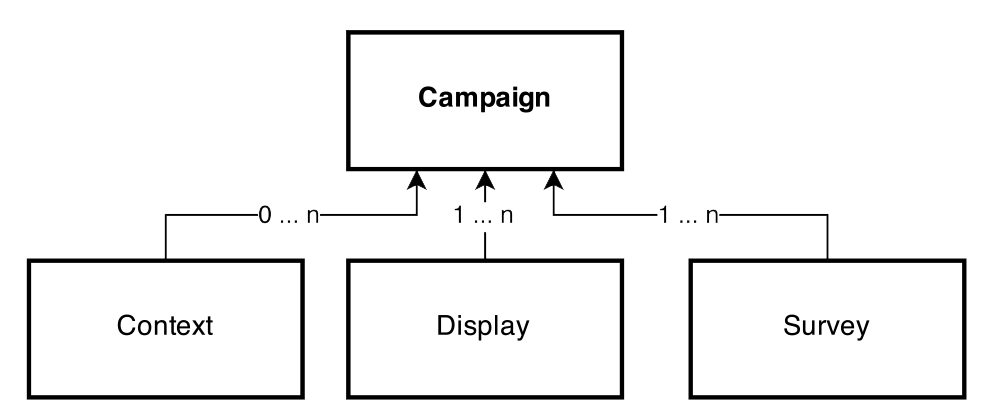
\includegraphics[width=.8\columnwidth]{img/4_implementation/4-dependency-campaign}
    \end{center}
 % \begin{center}\LARGE [BILD]\end{center}
 \caption{Campaign model dependencies}
 \label{fig:4-dependency-campaign}
\end{figure}


++ neue Namensgebung, um in der domain specific language zu bleiben --> application provider / display provider / space provider (anstatt Operator). Wir werden aber nur mit dem Application Provider (anstatt Operator) im System arbeiten




\subsubsection{User stories}

Concept from extreme programming.

\begin{enumerate}
\item inspired by: ...
\item criteria for good user stories: http://tigertechtalk.wordpress.com/2012/10/17/wie-schreibe-ich-eine-gute-user-story-und-was-ist-das-uberhaupt/
\end{enumerate}



+ User Centered Design (paper nr 31): ``constitutes an iterative process of system design, deployment and evaluation'' (quote from paper 31)






\subsubsection{User roles}

As of now only two roles are implemented, the admin-role and the guest-role.

% FEEDBACK VON FLORIAN: nein, nicht zu komplex machen. Es sollte sogar reichen, nur zwischen Admin & Operator (= Application Provider) zu unterscheiden, da der end user (das Public Display) ja sowieso nur auf die öffentlichen REST API Zugriff hat. (2014-11-14)


In the long term it would be desirable to have the following user roles: Admin, Operator, Evaluator, DisplayApplication.



\subsubsection{REST interface}

Defining the REST API. 

% TODO: Explain why I chose which level of separation / detail.

Notes from before I started writing
\begin{enumerate}
\item Think about using a Extreme Programming approach http://www.extremeprogramming.org/rules.html
\end{enumerate}